\chapter{Effet d'une \secpent sur les caractéristiques du \jat}\label{annexe:SectionPentue}
\minitoc

%\section{Ralentir un jet avec une pente}\label{sec:RalentirPente}
Dans cette annexe, nous présentons une modélisation \ude de la propagation d'un \jat le long d'une \secpent. 
Nous étudierons sa mise hors d'\eqthdy du jet, puis nous considèrerons la \reth de ce dernier en tenant compte des degrés de liberté transverses.

\RemarqueTitre{De manière qualitative \ldots}{
%\section{Augmentation de la \dispvitlong dans une \secpent}
On peut prévoir intuitivement que la \dispvitlong augmente lorsqu'un \jat gravit une pente. En effet, considérons les deux énergies en jeu, utiles à la compréhension du problème:
\begin{itemizel}
	\item l'énergie cinétique de chaque atome, qui est quadratique en vitesse: $E_c=\tfrac{1}{2}m v^2$,
	\item l'énergie potentielle de gravité, qui est linéaire en altitude $E_p \equiv m g z$. 
\end{itemizel}
En gravissant une hauteur $h$ donnée, chaque atome va convertir la même quantité d'énergie cinétique en énergie potentielle, ce qui va donc correspondre à une faible diminution de la vitesse d'un atome \sotosay{rapide}, alors que pour un atome \sotosay{lent} la diminution de vitesse doit être plus élevée (à cause du terme quadratique en vitesse). 

\noindent En conséquence, les atomes sont bien ralentis, mais pas tous de la même manière: les atomes \sotosay{rapides} vont un peu ralentir, et les atomes \sotosay{lents} vont beaucoup ralentir (voire rebrousser chemin), creusant ainsi l'écart entre les différentes vitesses au sein du \jat.
}

\casse

\section{Étude de  la mise hors d'équilibre du \jat}
Proposons-nous d'étudier de manière quantitative le problème de la mise hors d'équilibre du \jat lors de sa propagation dans la section pentue du guide. Nous désirons en fait prédire, dans le cadre d'un modèle simplifié, de quelle manière est modifiée la distribution de vitesses du jet.

Pour ce faire, nous allons modéliser le \jat par un système unidimensionnel de particules se propageant suivant l'axe $z$ de la \secpent du guide. L'origine de cet axe sera prise comme étant en bas de la pente. Avec pour objectif d'étudier la dynamique temporelle du problème, nous supposerons qu'à l'instant initial $t=0$ (voir la figure~\nref{fig:ModelPente}):
\begin{itemize}
	\item seule la partie horizontale précédant la \secpent est uniformément occupée par des particules avec une densité linéique $\Nlongini \equiv n(z \leq 0, t = 0)$,
 \item le jet dans l'espace $z<0$, est à l'\eqthdy avec une distribution gaussienne de vitesses décrite par une vitesse moyenne $\vjetini$ et une \templong $\Tlongini$. 
\end{itemize}
De plus, nous supposerons que les atomes n'interagissent pas, \cad que chacun d'eux gravit la pente indépendamment de la présence des autres atomes. On ne considère donc pour l'instant aucun processus de \reth.
\bfigs
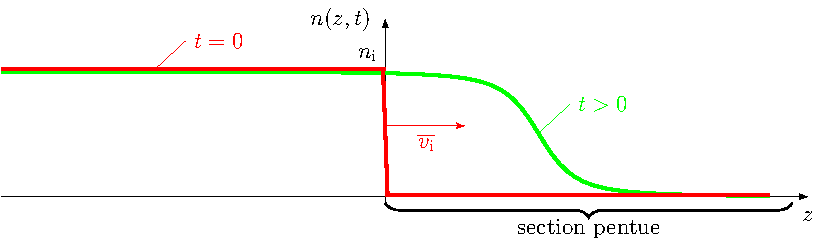
\includegraphics{P2/ModelPente}
%\RemonteUnPeuFig
\CaptionFigss{Représentation de la \datlin $n(z,t)$ à l'instant initial $t=0$, et à un instant ultérieur $t>0$.
L'origine de l'axe $z$ est prise comme étant en bas de la pente. \`A l'instant initial $t=0$ seule la partie horizontale précédant la \secpent est uniformément occupée par des particules avec une densité linéique $\Nlongini$. De plus, on considère un équilibre thermodynamique local avec une distribution gaussienne de vitesses décrite par une vitesse moyenne $\vjetini$ et une \templong $\Tlongini$.}
\label{fig:ModelPente}
\efig
La \fdddedpup à l'instant initial s'écrit donc:
\begin{equation}\label{eq:fiPente}
	f_i(z, v, t=0) = \sqrt{\frac{m}{2\,\pi\,\kb\,\Tlongini}} \, \Nlongini
	\,\Expo{-\frac{m\,\left( v - \vjetini \right)^2}{2\,\kb\,\Tlongini}} \Heaviside{-z}
	\pointformule
\end{equation}

Afin de calculer l'évolution de cette \fdd, il nous faut connaître les équations du mouvement dans la section pentue du guide. Une particule initialement en $z_0 \leq 0$ avec une vitesse $v_0 \geq 0$, atteindra la section pentue ($z=0$) du \gm à un temps $t_0 = \tfrac{-z_0}{v_0}$ et les équations donnant sa vitesse $v_p(t)$ et sa position $z_p(t)$ s'écrivent alors, dans la section pentue (donc pour $t \geq t_0$):
\begin{equation}
	\begin{cases}
	v_p(t) &= v_0 - \sinalpha \, g \, (t-t_0) \\
	z_p(t) &= v_0 \, (t-t_0) - \frac{\sinalpha \, g}{2} \, (t-t_0)^2
	\virguleformule
	\end{cases}
	\label{eq:MouvementPente}
\end{equation}
$\alpha$ étant l'angle entre l'axe $z$ du guide en pente et l'horizontale, et $g$ l'accélération de la pesanteur. En constatant que, si on ne considère que les particules pour lesquelles $v_p \geq 0$ (\cad les particules gravissant la pente), le système d'équations~\nref{eq:MouvementPente} est équivalent au système:
\begin{equation}
	\begin{cases}
	v_0 &= v_p \, \sqrt{1 + \frac{2 \, \sinalpha \, g \, z_p}{{v_p}^2}} \\
	z_0 &= 2\,z_p
	+\frac{{v_p}^2}{\sinalpha\,g}
	- \left(	{v_p}\,t + \frac{{v_p}^2}{\sinalpha\,g}  \right)
	\sqrt{1 + \frac{2\,\sinalpha\,g\,z_p}{{v_p}^2}}
	\virguleformule
	\end{cases}
	\label{eq:MouvementPenteBis}
\end{equation}
et nous pouvons ainsi calculer la \fdddedpup à un instant $t$ donné et en un point $z>0$ de la \secpent:
\begin{align}
	f_p(z\geq0, v\geq0, t) = 
	 \iint \ddint v_0 \ddint t_0 \, \,
	& f_i(z_0, v_0, t=0) 	 \nonumber \\
	& \Dirac{z_0 - 2\,z
	-\frac{{v}^2}{\sinalpha\,g}
	+ \left(	{v}\,t + \frac{{v}^2}{\sinalpha\,g}  \right)
	\sqrt{1 + \frac{2\,\sinalpha\,g\,z}{{v}^2}}}	 \nonumber \\
	& \Dirac{v_0 - v\,\sqrt{1 + \frac{2\,\sinalpha\,g\,z}{{v}^2}}} 
	\pointformule
	\label{eq:fpPente}
\end{align}

\Resultat{
Nous obtenons la \fdd du jet dans la \secpent ($z>0$, $v>0$, $t>0$):
\begin{align}
	f_p(z, v, t) = & 
	 \sqrt{\frac{m}{2\,\pi\,\kb\,\Tlongini}} \Nlongini 
	 \, \Expo{-\frac{m\,\left(v\,\sqrt{1 + \frac{2\,\sinalpha\,g\,z}{{v}^2}} - \vjetini \right)^2}{2\,\kb\,\Tlongini}} \nonumber \\
	&	\times \Heaviside{-2\,z
	-\frac{{v}^2}{\sinalpha\,g}
	+ \left(	{v}\,t + \frac{{v}^2}{\sinalpha\,g}  \right)
	\sqrt{1 + \frac{2\,\sinalpha\,g\,z}{{v}^2}}}
	\virguleformule
	\label{eq:fpPenteJat}
\end{align}
que l'on peut interpréter de la manière suivante: 
\begin{itemize}
	\item le terme $\Heaviside{\cdots}$ de Heaviside traduit l'établissement du régime stationnaire. Il contient les informations relatives aux corrélations position-temps-vitesse. On constate d'ailleurs qu'avec $t\rightarrow\infty$, ce terme vaut 1.
	\item le terme dans l'exponentielle donne les corrélations position-vitesse au sein du jet une fois le régime stationnaire établi dans la section pentue.
\end{itemize}
}
Cette \fdd du \jat nous permet de calculer la vitesse moyenne $\vjetfin$ et la \templong $\Tlongfin$ 
%(telle qu'elles sont définies par~\nref{eq:defTlong} et~\nref{eq:defVmoy} pour une distribution quelconque), 
mais ne donne pas de formulation analytique simple. Il faut noter d'ailleurs que l'expression de la \templong n'est pas d'un grand intérêt dans la mesure où la \fdd représente l'état d'un système loin de l'\eqthdy. Nous pouvons cependant considérer la \reth du \jat qui suit cette mise hors d'équilibre. Avant cela, faisons d'abord une simple application numérique pour nous rendre compte des ordres de grandeur des effets dont il est question:
\ApplicationNumerique{%
Prenons les caractéristiques typiques d'un \jat produit grâce à notre \setup:
\begin{itemize}
	\item vitesse moyenne du \jat, $\vjetini = \cmps{110}$,
	\item température longitudinale%
	\footnotemark, $\Tlongini = \microK{150}$,
	\item dénivellation de la pente, $\Hpente = \mm{22}$.
\end{itemize}

En intégrant numériquement l'équation~\nref{eq:fpPente} %, puis en appliquant les définitions de $\vjetfin$ et $\Tlongfin$% (équations~\nref{eq:defTlong} et~\nref{eq:defVmoy}), 
 nous obtenons en haut de la pente en régime stationnaire:
\begin{itemize}
	\item vitesse moyenne, $\vjetfin = \cmps{86}$ ,
	\item température longitudinale, $\Tlongfin = \microK{260}$.
\end{itemize}
}
\footnotetext{Rappelons que la \templong d'un \pat individuel est inférieure à la température d'\eqthdy du jet dont il est question dans le chapitre~\nref{chap:JetAtomique}. Ce point a été discuté dans la \autoref{sec:EntreeGuideNonAdiabatique}.}
C'est donc un effet important puisqu'en ralentissant le \jat d'un quart de sa vitesse, on double presque sa \templong dans les conditions typiques de notre \setup.

\section{Rethermalisation du \jat}
La \reth implique tous les degrés de liberté, et notamment les degrés de liberté transverses, sur lesquels le \gm impose un confinement. Pour toutes les expériences décrites dans ce chapitre, le \ppt est purement linéaire en distance à l'axe du \gm (voir \autoref{sec:PiegeageMagnetiqueGuide}).
Dans ces conditions, et en supposant que le \jat, au moment où il atteint la section pentue, est à l'équilibre \thdy défini par la température $\Teqini$, nous pouvons écrire l'énergie \thiq moyenne par particule dans le \gm avant la section pentue sous la forme:
\begin{equation}
\Moyenne{\Eatini} = \frac{7}{2}\,\kb\,\Teqini = 
	\ArriveeHiglightColorMath{blue}{3 \, \frac{\kb\,\Teqini}{2}}
	+ \ArriveeHiglightColorMath{red}{2 \, \kb\,\Teqini}
	\virguleformule
	\label{eq:EatiniPente}
\end{equation}
répartie sur \DepartHighlightColor{blue}{$3$ degrés de liberté} quadratiques en vitesse et \DepartHighlightColor{red}{$2$ degrés de liberté transverses} correspondant au \pctlin en distance à l'axe.
\MakeFlecheHighlightColor{blue}
\MakeFlecheHighlightColor{red}

\Remarque{\label{Rq:Viriel}
Ceci est un cas particulier d'application du théorème du viriel qui stipule que l'énergie moyenne d'une particule vaut:
\[
\epsilon = \frac{\kb\,T}{\delta} 
\virguleformule 
\]
sur chaque degré de liberté intervenant à la puissance $\delta$ dans l'expression de l'énergie mécanique du système. Par exemple, si l'énergie mécanique s'écrit:
\[
\Ham(\Vecteur{r},\Vecteur{v}) = \frac{1}{2}\,m\,\left( {v_x}^2 + {v_y}^2 + {v_z}^2 \right) + \alpha \Module{x}^3 + \beta \Module{y} 
\virguleformule
\]
alors l'énergie moyenne d'une particule faisant partie d'un système caractérisé par une température $T$ est :
\[
\Moyenne{\Eat} \equiv \MoyenneBraKet{\Ham} = \frac{\kb\,T}{2} + \frac{\kb\,T}{2} + \frac{\kb\,T}{2} + \frac{\kb\,T}{3} + \kb\,T 
\pointformule
\]
\finformule
%où $\MoyenneBraKet{\Ham}\equiv\frac{
%\Integrale{\Ham\,\expo{-\ttfrac{\Ham}{\kb\,T}}}{\dd^3r\,\dd^3v}}{
%\Integrale{\expo{-\ttfrac{\Ham}{\kb\,T}}}{\dd^3r\,\dd^3v}}$.
}

Lorsque les particules gravissent la pente, l'une des composantes de la température, $\Tlong$, augmente de $\Delta \Tlong \equiv \Tlongfin - \Teqini$. La conservation de l'énergie \thiq moyenne par particule lors de la \reth au delà de la section pentue nous donne la température $\Teqfin$ à laquelle le \jat va rethermaliser:
\begin{equation}
\Moyenne{\Eatfin} \equiv 
	\ArriveeHiglightColorMath{red}{\frac{7}{2}\,\kb\,\Teqfin}
	= \ArriveeHiglightColorMath{blue}{2\,\frac{\kb\,\Teqini}{2}	+ \frac{\kb\,\Tlongfin}{2} + 2\,\kb\,\Teqini}
	= 3\,\kb\,\Teqini + \frac{\kb\,\Tlongfin}{2}
\pointformule
	\label{eq:PenteRetherm}
\end{equation}
Cette égalité rappelle l'équation~\nref{eq:EatiniPente} mais porte sur une situation hors d'\eqthdy en haut de la section pentue \DepartHighlightColor{blue}{avant \reth} et une situation d'équilibre \DepartHighlightColor{red}{après \reth.}
%\MakeFlecheHighlightColor{blue}
%\MakeFlecheHighlightColor{red}
 Nous déduisons donc la température d'équilibre au delà de la section pentue:
\begin{equation}
	\Teqfin = \Teqini + \frac{\Delta \Tlong}{7}
	\label{eq:PenteRethermTeq}
\pointformule
\end{equation}
La variation de \templong liée au fait que le \jat gravit une pente sera donc réduite par un facteur $7$ après \reth, du fait de la redistribution sur tous les degrés de liberté.

\RemarqueTitre{Ralentir un paquet avec une pente}
{\label{Rq:RalentirPaquetPente}
Si on considère l'évolution d'un seul \pat gravissant la \secpent, les équations du mouvement~\nref{eq:MouvementPente} restent valables. On peut montrer qu'en appliquant la formule~\nref{eq:fpPente} on aboutit à un résultat similaire à~\nref{eq:fpPenteJat}, \cad que la \dispvitlong du \pat augmente lorsque celui-ci gravit une pente.
}
